\chapter{Smart Railway Communication System}

Gradually we are moving towards context awareness among automotive devices, where the vehicles are aware of their neighborhood. In modern trains a huge amount of wireless communications are used for safety features like train collision avoidance, railway management or customer oriented services such as passenger Internet access. To enhance reliability and safety of Railway systems while increasing accessibility and productivity, modern railway operations rely on ever increasing exchanges of information between the different wireless communication in terms of train-to-train (T2T) and train-to-ground (T2G). The integration of all the heterogeneous wireless networks deployed in the railway domain constitutes a key technical challenge. This can be answered by emerging Cognitive Radio (CR) technologies which can offer interoperability, reliability, dynamic spectrum access and lower deployment, and maintenance cost. The research is underway for cognitive radio enabled railway communication and two most famous projects are:

\begin{itemize}

\item Cognitive Radio for Railway Through Dynamic and Opportunistic Spectrum Reuse (CORRIDOR)~\cite{corridor} is a French research project that targets opportunistic spectrum access for railways. Due to rapid increase in demand for future railways in terms of control operations as well as providing high speed internet connectivity to the passengers, more bandwidth and spectrum is needed for railway communication.

\item Rail-CR project~\cite{5621621} is a US-based Railway system project where the main effort is to implement a positive train control (PTC) technology to equip trains with wireless communication capabilities. The project aims to allow trains to communicate with wayside wireless stations, while moving to supply important information like speed, direction, etc. to improve safety and operations of the railways.

\end{itemize}

In the following section we discuss positive train control (PTC), wireless broadband (WiBro), train-to-train (T2T) and train-to-ground (T2G) communication, Long Term Evolution for Railways (LTE-R) communication system, spectrum regulation for LTE-R, LTE and Internet-of-Things (IoT) for railways which are important technologies for achieving smart railway transportation system.

\section{Positive Train Control}
Positive Train Control (PTC) is an advanced system designed for monitoring and controlling of train movements to provide advanced safety with the help of modern wireless communication technology. The key idea behind PTC is the constant flow of information to the train about its location, warnings if engineer doesn't slow down the train, derailments caused by excessive speed of train, etc. Managing track occupancies through centralized route and interlocking logic, enforcing permanent and temporary speed limits for the train, real-time localization of the train these are some of the basic features implemented in PTC. 

\begin{figure}[!ht]
\centering
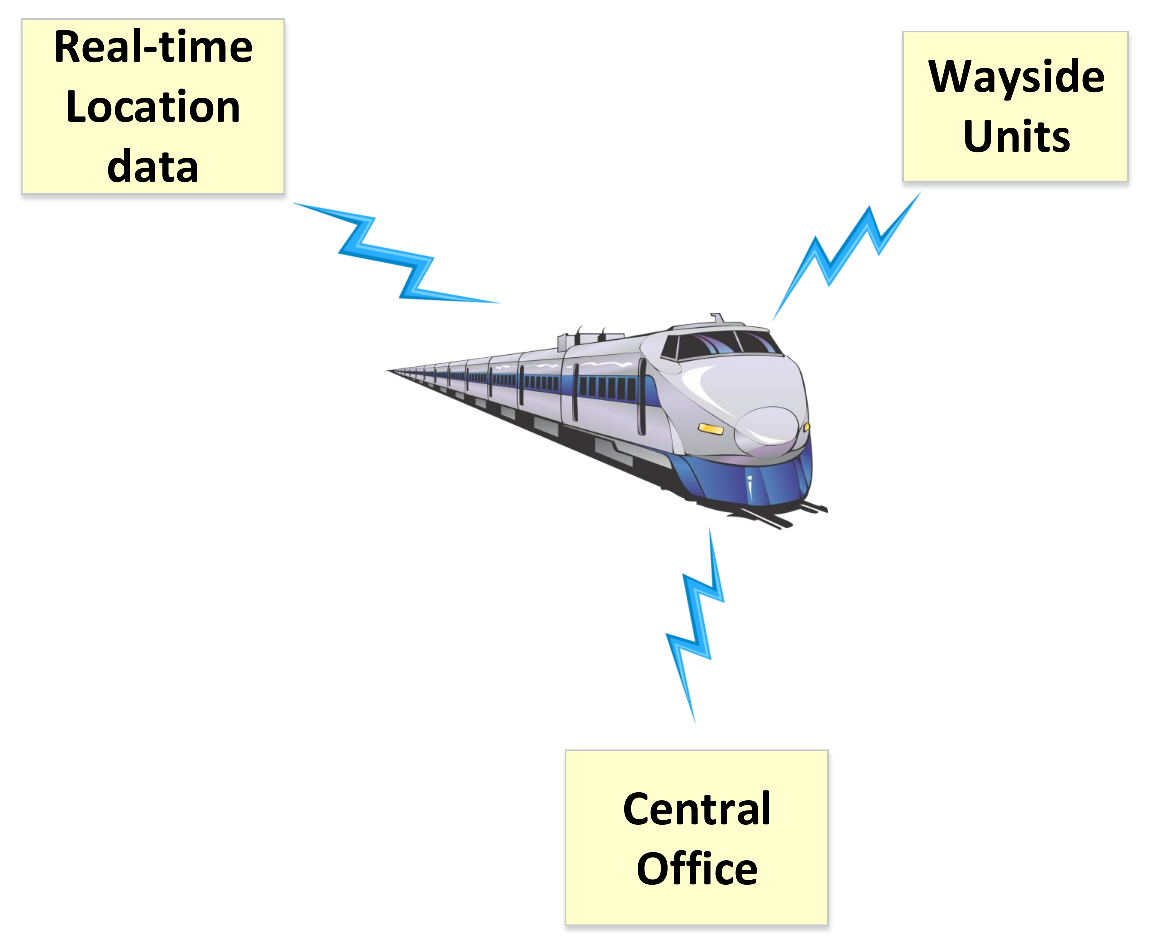
\includegraphics[width=\textwidth,height=10cm,keepaspectratio]{images/Gill/5G/ptc.eps} 
\caption{Architecture of Positive Train Control}
\label{ptc}
\end{figure}


The Figure~\ref{ptc} gives the simplistic architecture of the PTC, where train receives the flow of information through various system using wireless communication links. The primary means of determining location for the train is by using differential GPS which can continuously compare it's position with the stored position of speed restriction and work zones~\cite{5338992}. Central Office (CO) regularly monitor trains, exchanging information with Train management computers (TMC) and gathering precise speed and position information. CO also collects information regarding train orders, number of cars, weight, route and track characteristics along the route, including speed restrictions, curves, grades and crossing. All wayside equipments are continuously monitored by PTC, where it issue alerts in cases such as when an automatic crossing gate is not working or a hot box detector some axles slightly above a certain temperature level. It also applies corrective action in cases where there are reports of a possible track breakage due to extreme heat or a flood.

\section{Wireless Broadband (WiBro)}

Wireless Broadband (WiBro) is a mobile broadband wireless access (BWA) service which had its first public demonstration in Dec. 2005 and has been in service in South Korea since June 2006. WiBro was developed as a mobile BWA solution in Korea and was based on IEEE 802.11e WiMax standard. It is a subset of consolidated version of IEEE Standard 802.16-
2004 (fixed wireless specifications), P802.16e (enhancements to support mobility), and P802.16-2004/Cor1 (corrections to IEEE Standard 802.16-2004). The pro-files and test specifications of WiBro will be harmonized with WiMAX Forum’s mobile WiMAX profiles and test specification, drawing a convergence of the two standards.


\begin{figure}[!ht]
\centering
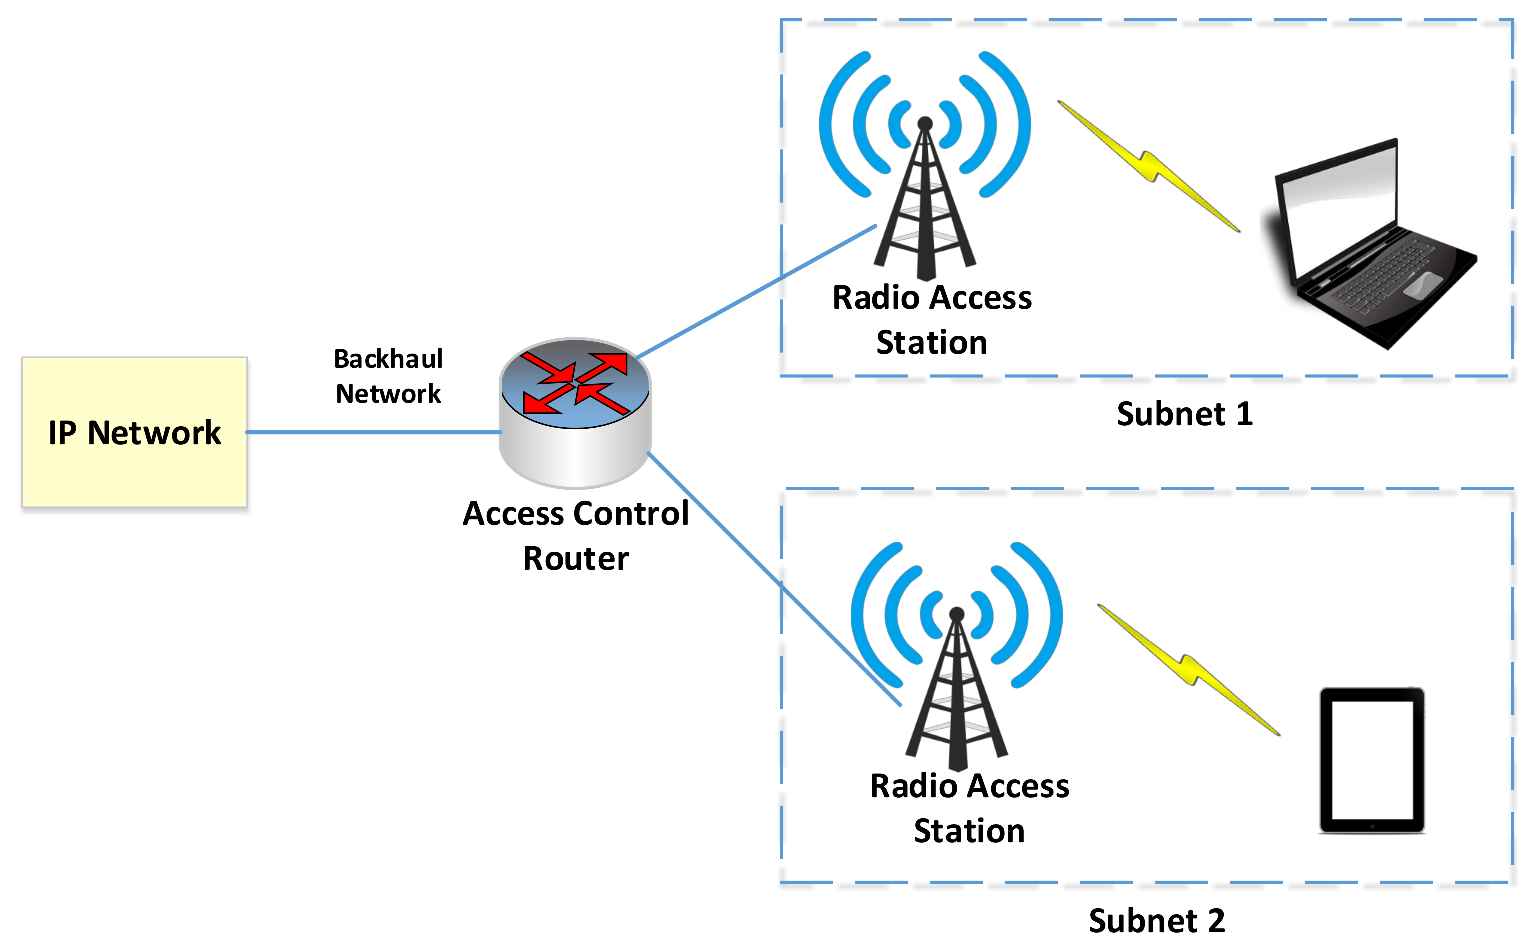
\includegraphics[width=\textwidth,height=10cm,keepaspectratio]{images/Gill/5G/wibro.eps} 
\caption{Korean Wireless Broadband (WiBro) system architecture for high speed internet connectivity.}
\label{wibro}
\end{figure}

Figure~\ref{wibro} describes the architecture of BWA based WiBro communication system in the phase I standardization~\cite{wibro}. The WiBro network consists of Access control Routers (ACR) which connects backbone network with Radio Access Station (RAS). The RAS is the interface between mobile nodes and the core network at the physical layer and it controls the radio resource at the data link layer in conjunction with an ACR. The key distinction of WiBro from conventional cellular networks is that Internet Protocol (IP) is used between an ACr and RASs and also between ACRs. WiBro uses Time or Frequency Division Duplexing (TDD or FDD) for duplexing and Orthogonal Frequency Division Multiple Access (OFDMA) for robustness against fast fading and narrow-band co-channel interference.


\section{LTE-R Communication System}

In recent years, the use of trains have witnessed tremendous growth due to their increasing speeds, which has led to the demand for reliable wireless communication systems with these transportation systems. The development of a reliable wireless network for high speed trains is not a simple task and it is still an emerging technology. Global System for Mobile
Communication (GSM-R)~\cite{trlter1}, was a wireless communications standard designed for high speed trains, but it turned out not to be reliable enough and possess several limitations. The data rate of voice services which can reach up to 9.6 kbps, which can't meet the increasing demands of high-rate data transmission in railways communication. The limited data rate and quality of service (QoS) is not enough to support cellular communication for current generation. These reasons have made the evolution of high speed railway communication more and more urgent.  Subsequently, LTE~\cite{trlter2} proposed a promising solution for achieving broadband data rates, flexible bandwidth allocation and high spectral efficiency in high speed trains that can overcome various GSM-R limitations~\cite{arlter3,inplter4}.

\begin{figure}[!ht]
\centering
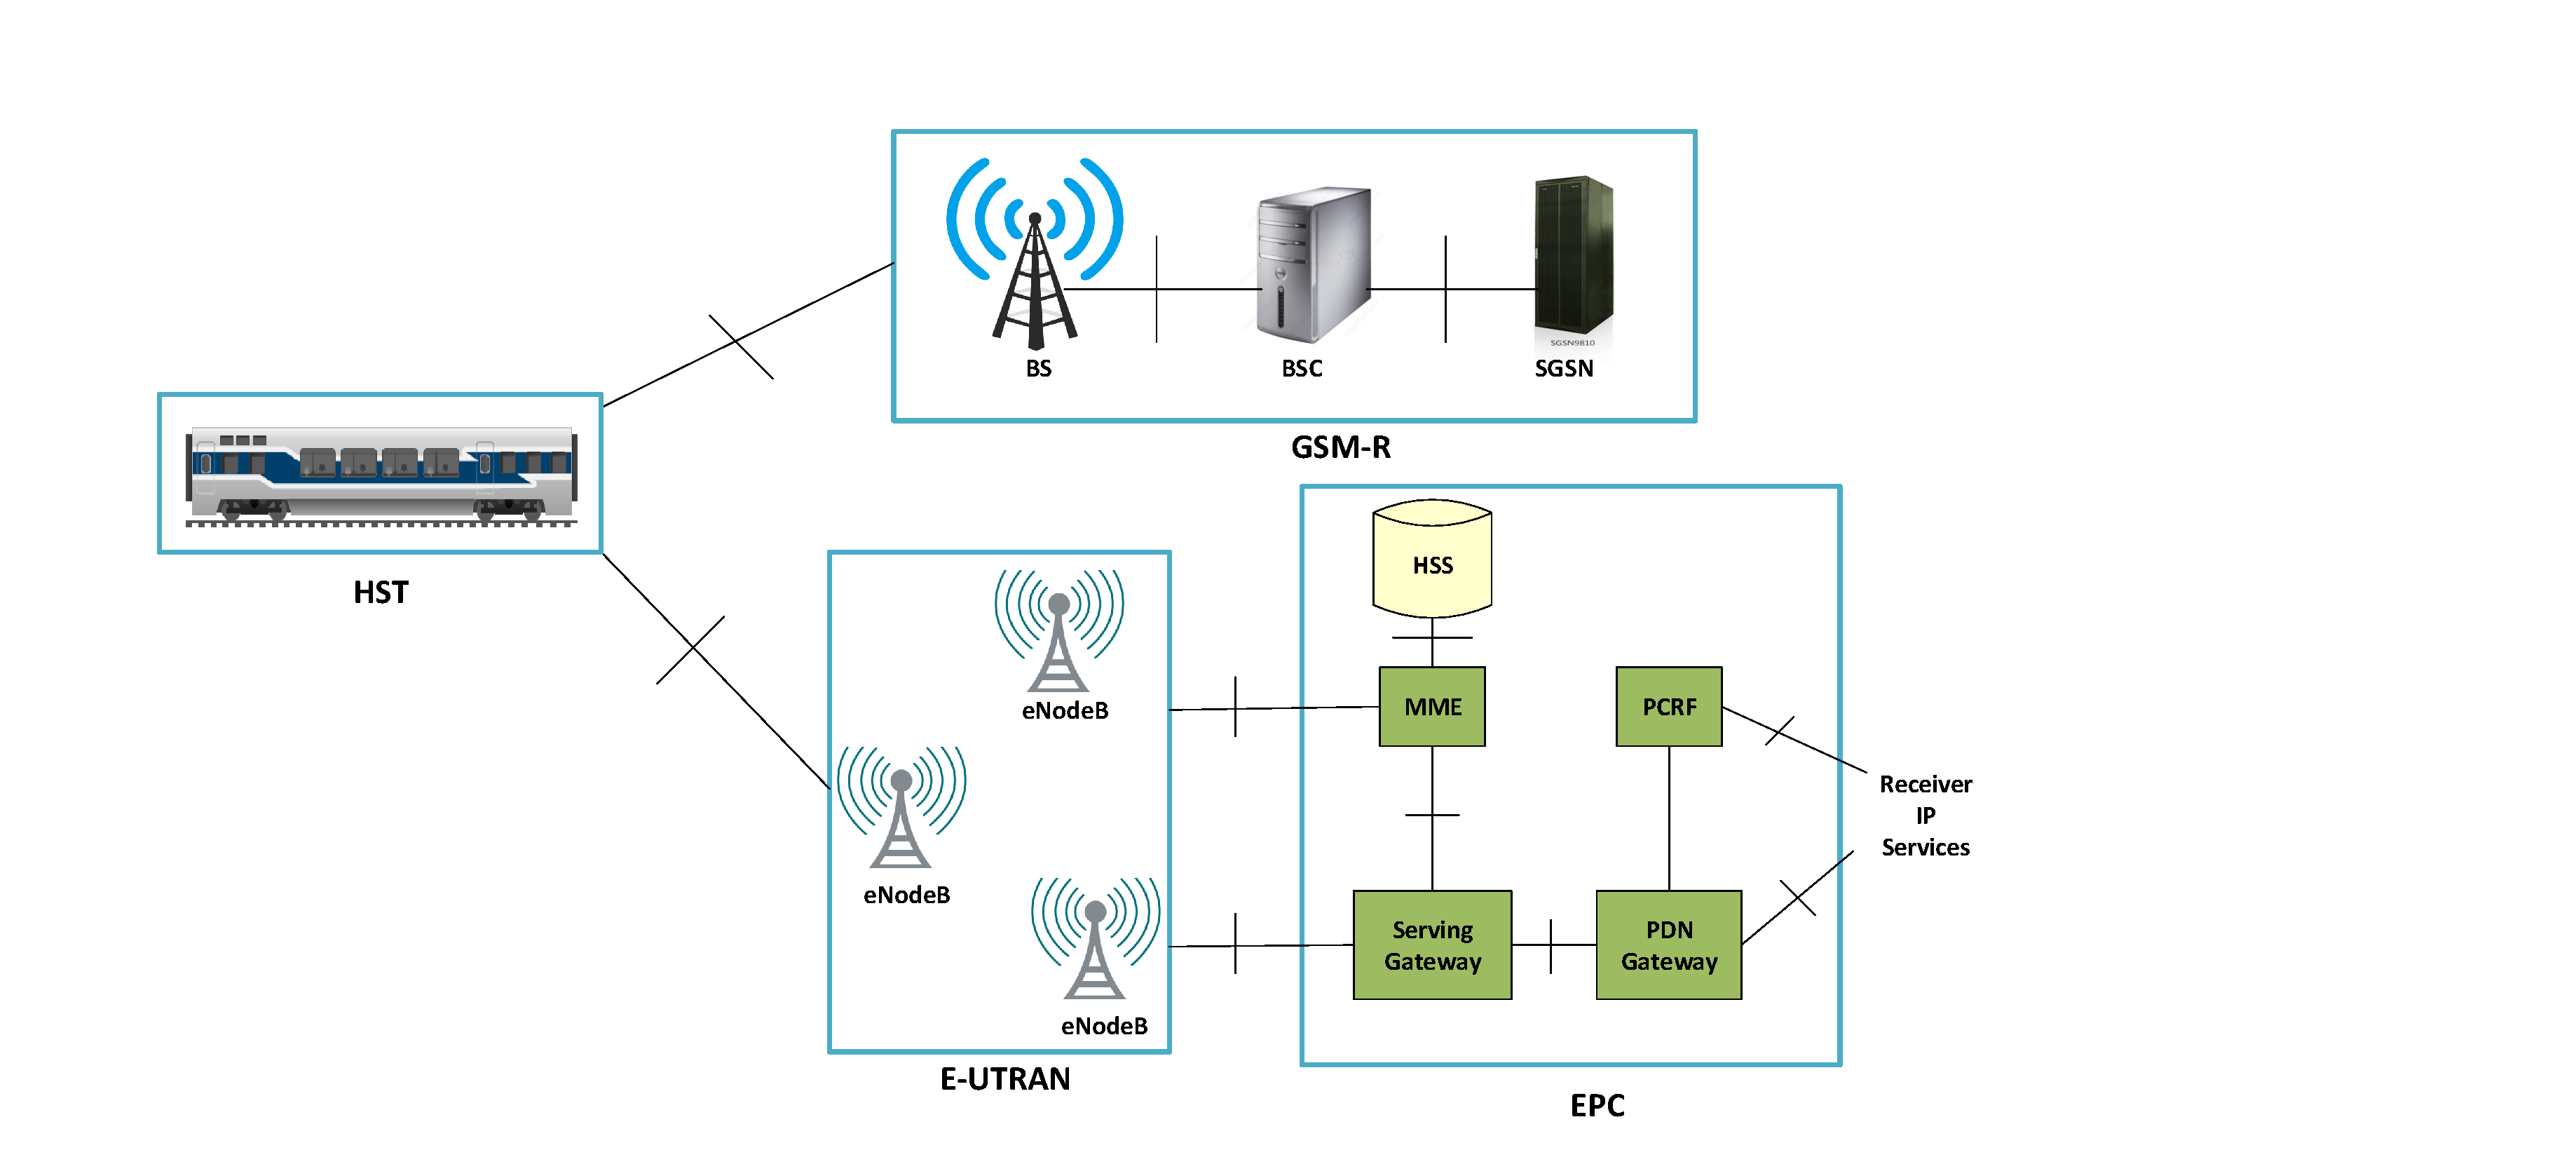
\includegraphics[width=\textwidth,keepaspectratio]{images/Gill/lte_figs/lter_architecture.eps} 
\caption{Proposed LTE-R Architecture for next generation High-speed Railways consisting of EPA and E-UTRAN.}
\label{ltearch}
\end{figure}

LTE-R is a high speed communication standard based on the existing LTE system architecture~\cite{inplter4}. There has been several studies regarding the assessment of LTE-R as a viable choice for next generation high speed communications for railway applications{inplter5,inplter6}. Conventional LTE includes a core network of evolved packet core (EPC) and a radio access network of Evolved Universal  Terrestrial  Radio  Access  Network (E-UTRAN). The  Internet  protocol (IP)-based  EPC  supports  seamless handovers for both voice and data to cell towers, and each E-UTRAN cell will support high data and voice capacity by high-speed  packet  access  (HSPA).  As  a  candidate for the next-generation  communication  system  of  HSR,  LTE-R  inherits all the important features of LTE and provides an extra radio access system to exchange wireless signals with onboard  units (OBUs)  and to match HST-specific  needs. Figure~\ref{ltearch} shows the proposed architecture of LTE-R according to~\cite{trlter2}, and it shows that the core network of LTE-R is backward compatible with GSM-R. The network architecture of LTE-R is similar to that of LTE/SAE with  Evolved Universal Terrestrial Radio Access Network (E-UTRAN) being the access network structure of LTE-R. There is evolved-Node B (eNodeB) that communicates directly with UEs like base transceiver station (BTS) in GSM network. It performs the transmission and reception of data packets using orthogonal frequency division multiplexing access (OFDM) for downlink and single carrier  frequency division multiple access (SC-FDMA) for uplink at PHY layer. At the same time, as without base-station controller (BSC), it also has functions of  radio  resource  control and wireless  mobility  management.  The eNodeBs can be connected to network router directly without more intermediate control nodes, such as the BSC in GSM-R~\cite{tingting2010high}. The core network of LTE-R is the Evolved Packet Core (EPC). The significant difference between EPC and the core network of GSM-R is that the EPC is an all-IP mobile core network.

\begin{table}[h!]
\caption{Comparison of system parameters between GSM-R , LTE and LTE-R.}
\begin{adjustbox}{width=1.22\textwidth, center=\textwidth}
\begin{tabular}{c | c | c | c}
\toprule
System Parameters & GSM-R & LTE & LTE-R\\ 
\midrule
Frequency & \shortstack{Uplink: 876--880 MHz\\downlink: 921--925 MHz} & 800, 1800, 2600 MHz & 450, 800, 1400, 1800 MHz \\  
Capacity  & 0.2 MHz & 1.4-20 MHz & 1.4-20 MHz\\ 
Modulation  & GMSK & QPSK/16-QAM/64-QAM & QPSK/16-QAM\\ 
MIMO  & No  & 2x2, 4x4  & 2x2\\ 
Cell Range  & 8 Km  & 1-5 Km & 4-12 Km \\ 
Data Rates (DL/UL)  & 172/172 Kbps  & 100/50 Mbps & 50/10 Mbps\\ 
\bottomrule
\end{tabular}
\end{adjustbox}
\label{ltertable}
\end{table}

Conventional LTE networks are different compared to LTE-R in many ways such as architecture, system parameters, network layout, services and quality of service (QoS). Table~\ref{ltertable} summarizes the LTE-R parameters and describe the differences between LTE, GSM-R and LTE-R. Since the LTE-R environment has very severe fading and high Doppler shift, it is configured for QoS rather than higher data rates. Therefore, QPSK modulation is used for most number of subcarriers and the number of packet re-transmission must be kept low and achieved with user datagram protocol (UDP).


\section{Spectrum Regulation for LTE-R}

Departing from technical issues, we now discuss the crucial interactions that smart railways will encounter with spectrum policy and allocation by the federal communications commission (FCC). As already discussed in Section~\ref{5gcell} the spectrum allocated for cellular technologies is already saturated in peak markets due to massive amounts of wireless services and networks. Figure~\ref{specalloc} shows the pronounced scarcity in the the wireless cellular bands as seen in the FCC frequency allocation chart. Large amount of unused spectrum is available in the mm-Wave realm and can be used for high data rate applications. Due to different propagation characteristics for signals at low and sub-terahertz frequencies, future systems will need to integrate a broad range of frequencies. Frequencies on a lower spectrum can be used for wide coverage, mobility support, control signaling and high frequencies for high data rate applications in small cells. This requires a new approach to spectrum policy and allocation methods for 5G standardization.

\begin{figure}[!ht]
	\centering
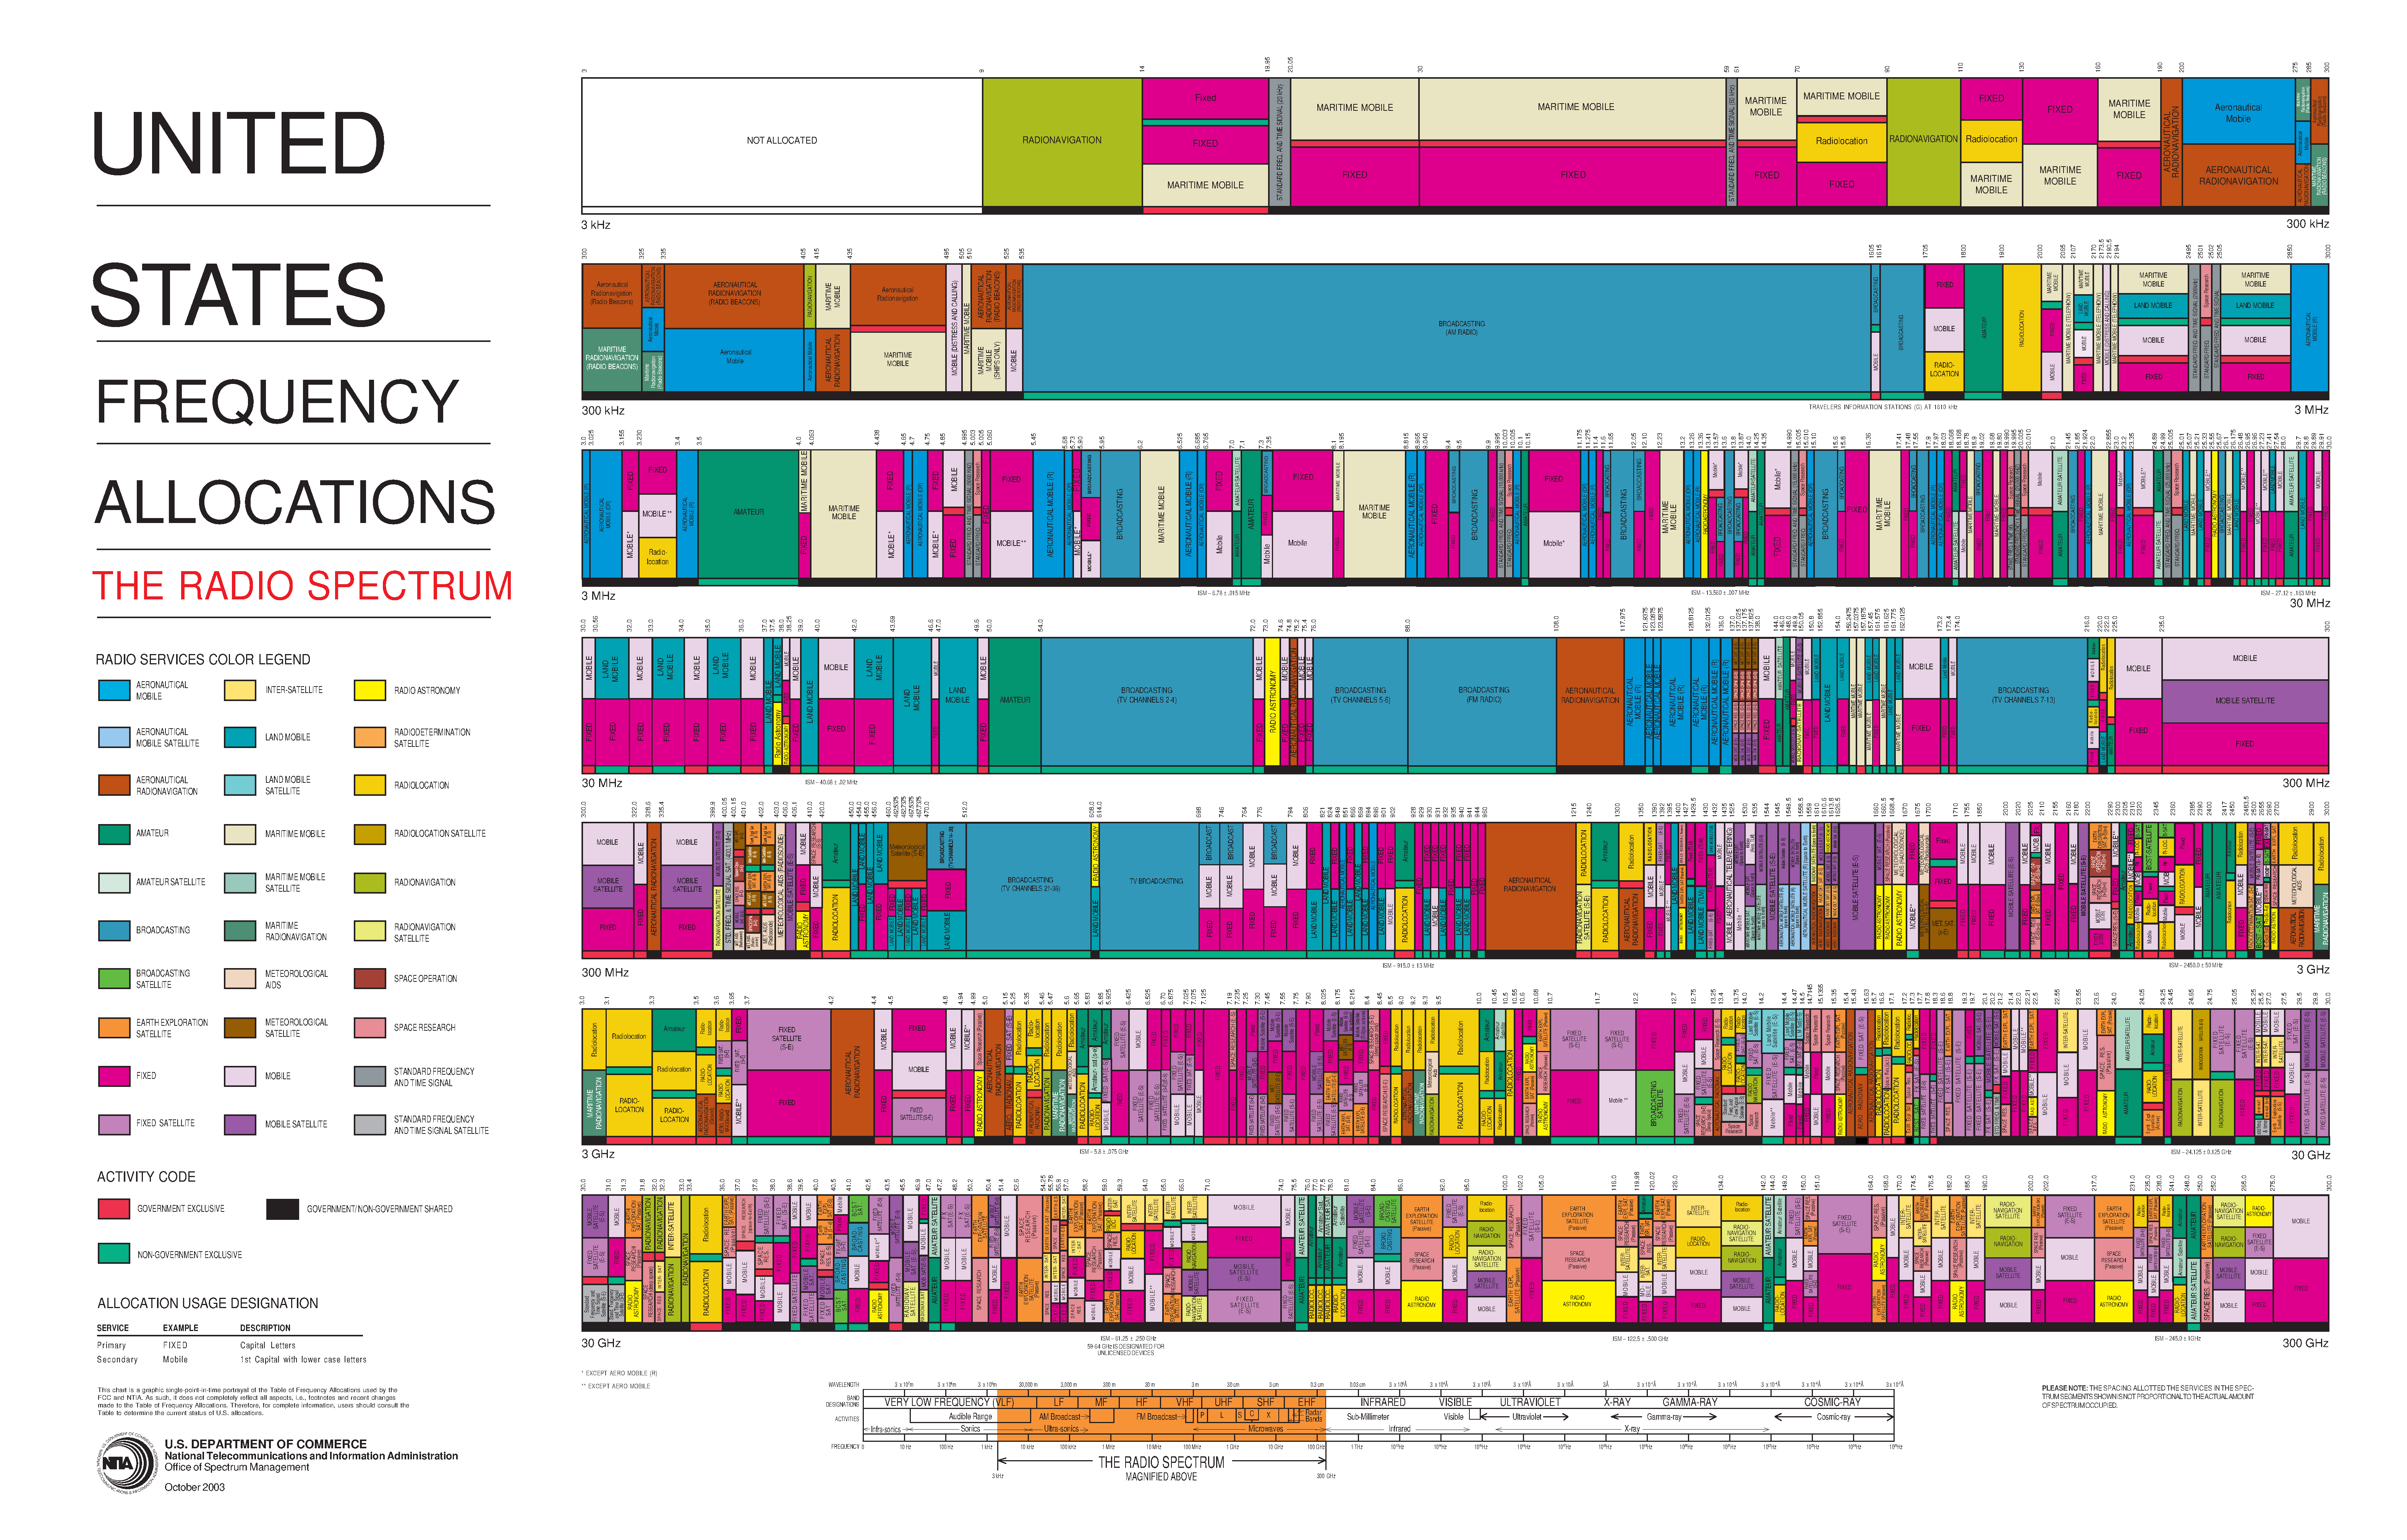
\includegraphics[width=\textwidth,keepaspectratio]{images/Gill/5G/specalloc.eps}
	\caption{Machine-to-Machine communication paradigm in 5G Cellular System.}
	\label{specalloc}
\end{figure}

Cognitive radio is a promising technology that can solve the spectrum shortage problem arising due to the rapid increase in wireless networks and mobile devices. Recent advancements in software-defined radio technology and edge computing have enhanced the cognitive radio network (CRN)  capabilities and, along with some adjustments in its operation, will be a key technology for 5G heterogeneous network deployment.  The CR network is an innovative software-defined radio technique considered to be one of the key technologies to improve the utilization of the congested radio spectrum~\cite{rusek2013scaling}. Integrating CR technology into 5G system is motivated by the fact that a large portion of the radio spectrum is underutilized most of the time. For achieving data rates in order of gigabits per second, we need to make an efficient use of available spectrum which can be achieved by utilizing CRNs. In CR networks, a secondary system can share spectrum bands with the incumbent primary system, either on an interference-free basis or on an interference-tolerant basis. The CR network should be aware of
the surrounding radio environment and regulate its transmission accordingly. In interference-free CR networks, CR users are allowed to borrow spectrum resources only when licensed users do
not use them. A key to enabling interference-free CR networks is figuring out how to detect the spectrum holes (white space) that spread out in wideband frequency spectrums and facilitate dynamic spectrum access (DSA) smoothly~\cite{wyglinski2009cognitive}. 

CR receivers should first monitor and allocate the unused spectrum via spectrum sensing (energy detection (ED), covariance absolute value (CAV) detection, etc.) or combining with geolocation databases and feed this information back to the central CR controller. A coordinating mechanism is required in multiple CR networks that try to access the same spectrum to prevent users colliding when accessing the matching spectrum holes. In interference-tolerant CR networks, CR users can share the spectrum resource with a licensed system while keeping the interference below a threshold. In comparison with interference-free CR networks, interference-tolerant CR networks can achieve enhanced spectrum utilization by opportunistically sharing the radio spectrum resources with licensed users, as well as better spectral and energy efficiency. However, it has been shown that the performance of CR systems can be very sensitive to any slight change in user densities, interference threshold, and transmission behaviors of the licensed system. However, the spectral efficiency can be improved by either relaxing the interference threshold of the primary system or considering only the CR users who have short distances to the secondary BS (utilizing the spatial gain). Hybrid CR networks have been proposed in~\cite{hong2010capacity} for adoption in cellular networks to explore additional bands and expand the capacity. CR networks can only prove beneficial if the spectrum policies related to 5G are implemented in a robust manner. 

\section{Vehicular Communication Using LTE}
With the development of mm-Wave and massive-MIMO, the spectral and energy efficiency for 5G wireless communications has been drastically improved. The development of driverless cars has posed some rigorous requirements for the safety of the passengers and pedestrians. For safety-critical applications the transmission delay needs to be less than 1 ms which is required for intelligent transportation systems (ITSs) and vehicular networks~\cite{ge2016vehicular}. Considering the drawbacks of IEEE 802.11p networks, such as poor scalability, low capacity , and intermittent connectivity, the Long Term Evolution (LTE) mobile communication technologies were proposed to support vehicular applications~\cite{araniti2013lte}. Simulation and experiment results revealed that there is a trade-off between the proposed performance metrics and system parameters, such as base station (BS) and vehicle densities, radio coverage, and  the  maximum  number of hops in a path. When LTE communication technologies have been integrated into vehicular networks, the interference has cut down the performance of LTE vehicular networks. When vehicle density is high, the beaconing signals of vehicular safety applications may easily overload the serving eNodeB. To handle this issue, a significant amount of such signals should be distributed directly among vehicles, without  going  through  the  eNB. In  LTE-Advanced (LTE-A), device-to-device (D2D) communication is considered to allow direct message delivery between terminals in proximity to lighten the load of eNB~\cite{mumtaz2014direct}. 

\begin{figure}[!ht]
	\centering
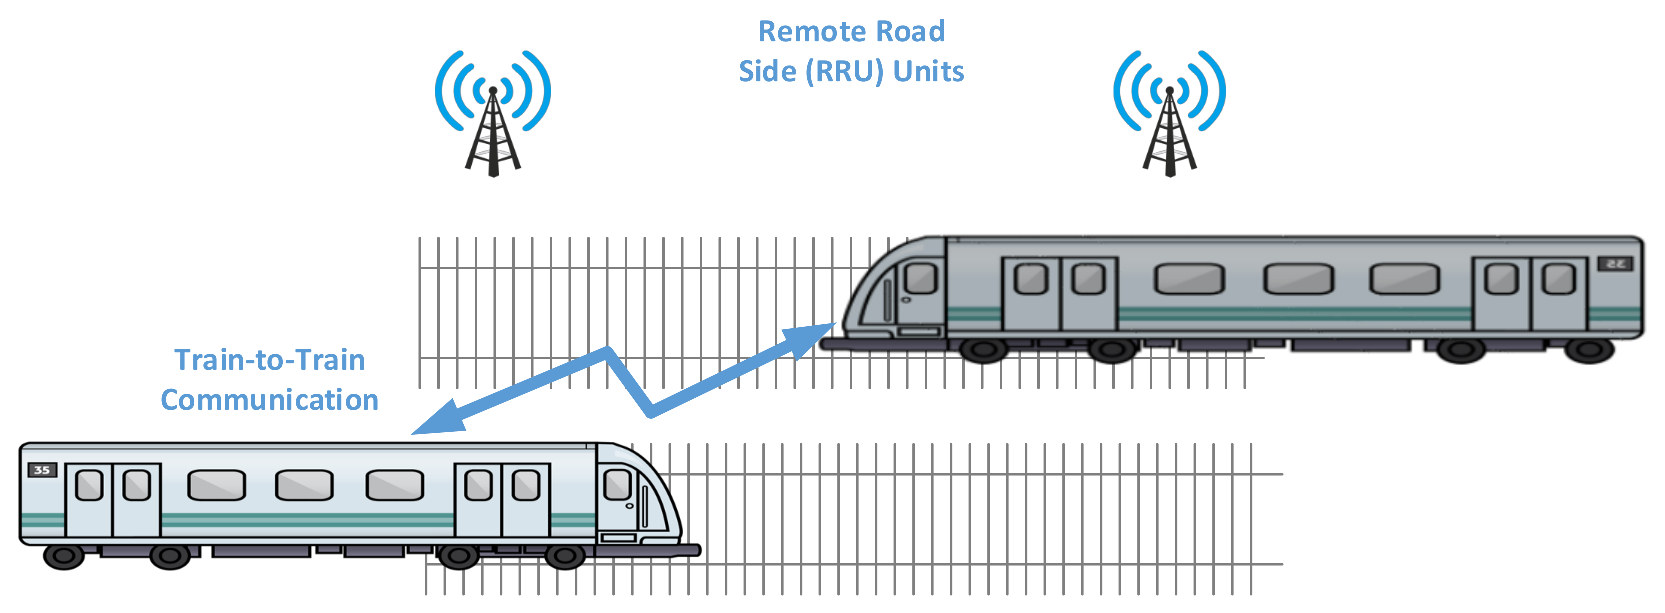
\includegraphics[width=\textwidth,keepaspectratio]{images/Gill/5G/vehiclecomm.eps}
	\caption{Vehicular communication using D2D 5G cellular communication technology.}
	\label{vcomm}
\end{figure}

Hence the infrastructure-aided D2D technologies can serve as a natural approach to enable reliable and efficient V2V communications without negatively affecting existing cellular systems. To meet the high performance requirements, such as low transmission delay and high throughput, a new architecture for 5G vehicular communication is required. Figure~\ref{vcomm} describes the vehicular communication  using D2D communication strategy where significant amount of computation is offloaded from road side units (RSU) to vehicles to avoid increase spectral and efficiency. The communication environment in V2V is quite different than in D2D due to high mobility (Doppler shift) of vehicles. Network connectivity play a important role in V2V communication than D2D, compared with system throughput. These features can significantly affect D2D resource allocation strategies and system parameters, and thus should be modified for vehicular communication.

\subsection{Internet of Things (IoT) for Railways}

Machine to machine (M2M) communication is a new paradigm proposed to be a key technology in 5G wireless systems that enables the ubiquitous connectivity  between a set  of devices  with different network stack.  Thus,  the  autonomous  connection  of  devices  facilitates  the  emergence  of  a  wide  range  of  intelligent M2M applications. M2M exhibits a strong potential to improve human life in different fields such as e-Health, smart  grids, smart cities, intelligent transportation and surveillance enabling internet of things (IoT) applications. A native inclusion of M2M communication in 5G involves satisfying three fundamentally different requirements associated with different classes of low data rates and power consumption services such as: enabling massive number of low-rate devices simultaneously, a minimal data rate in virtually all scenarios, even in worst fading environment and finally managing the above two requirements with a very low latency.


\begin{figure}[!ht]
	\centering
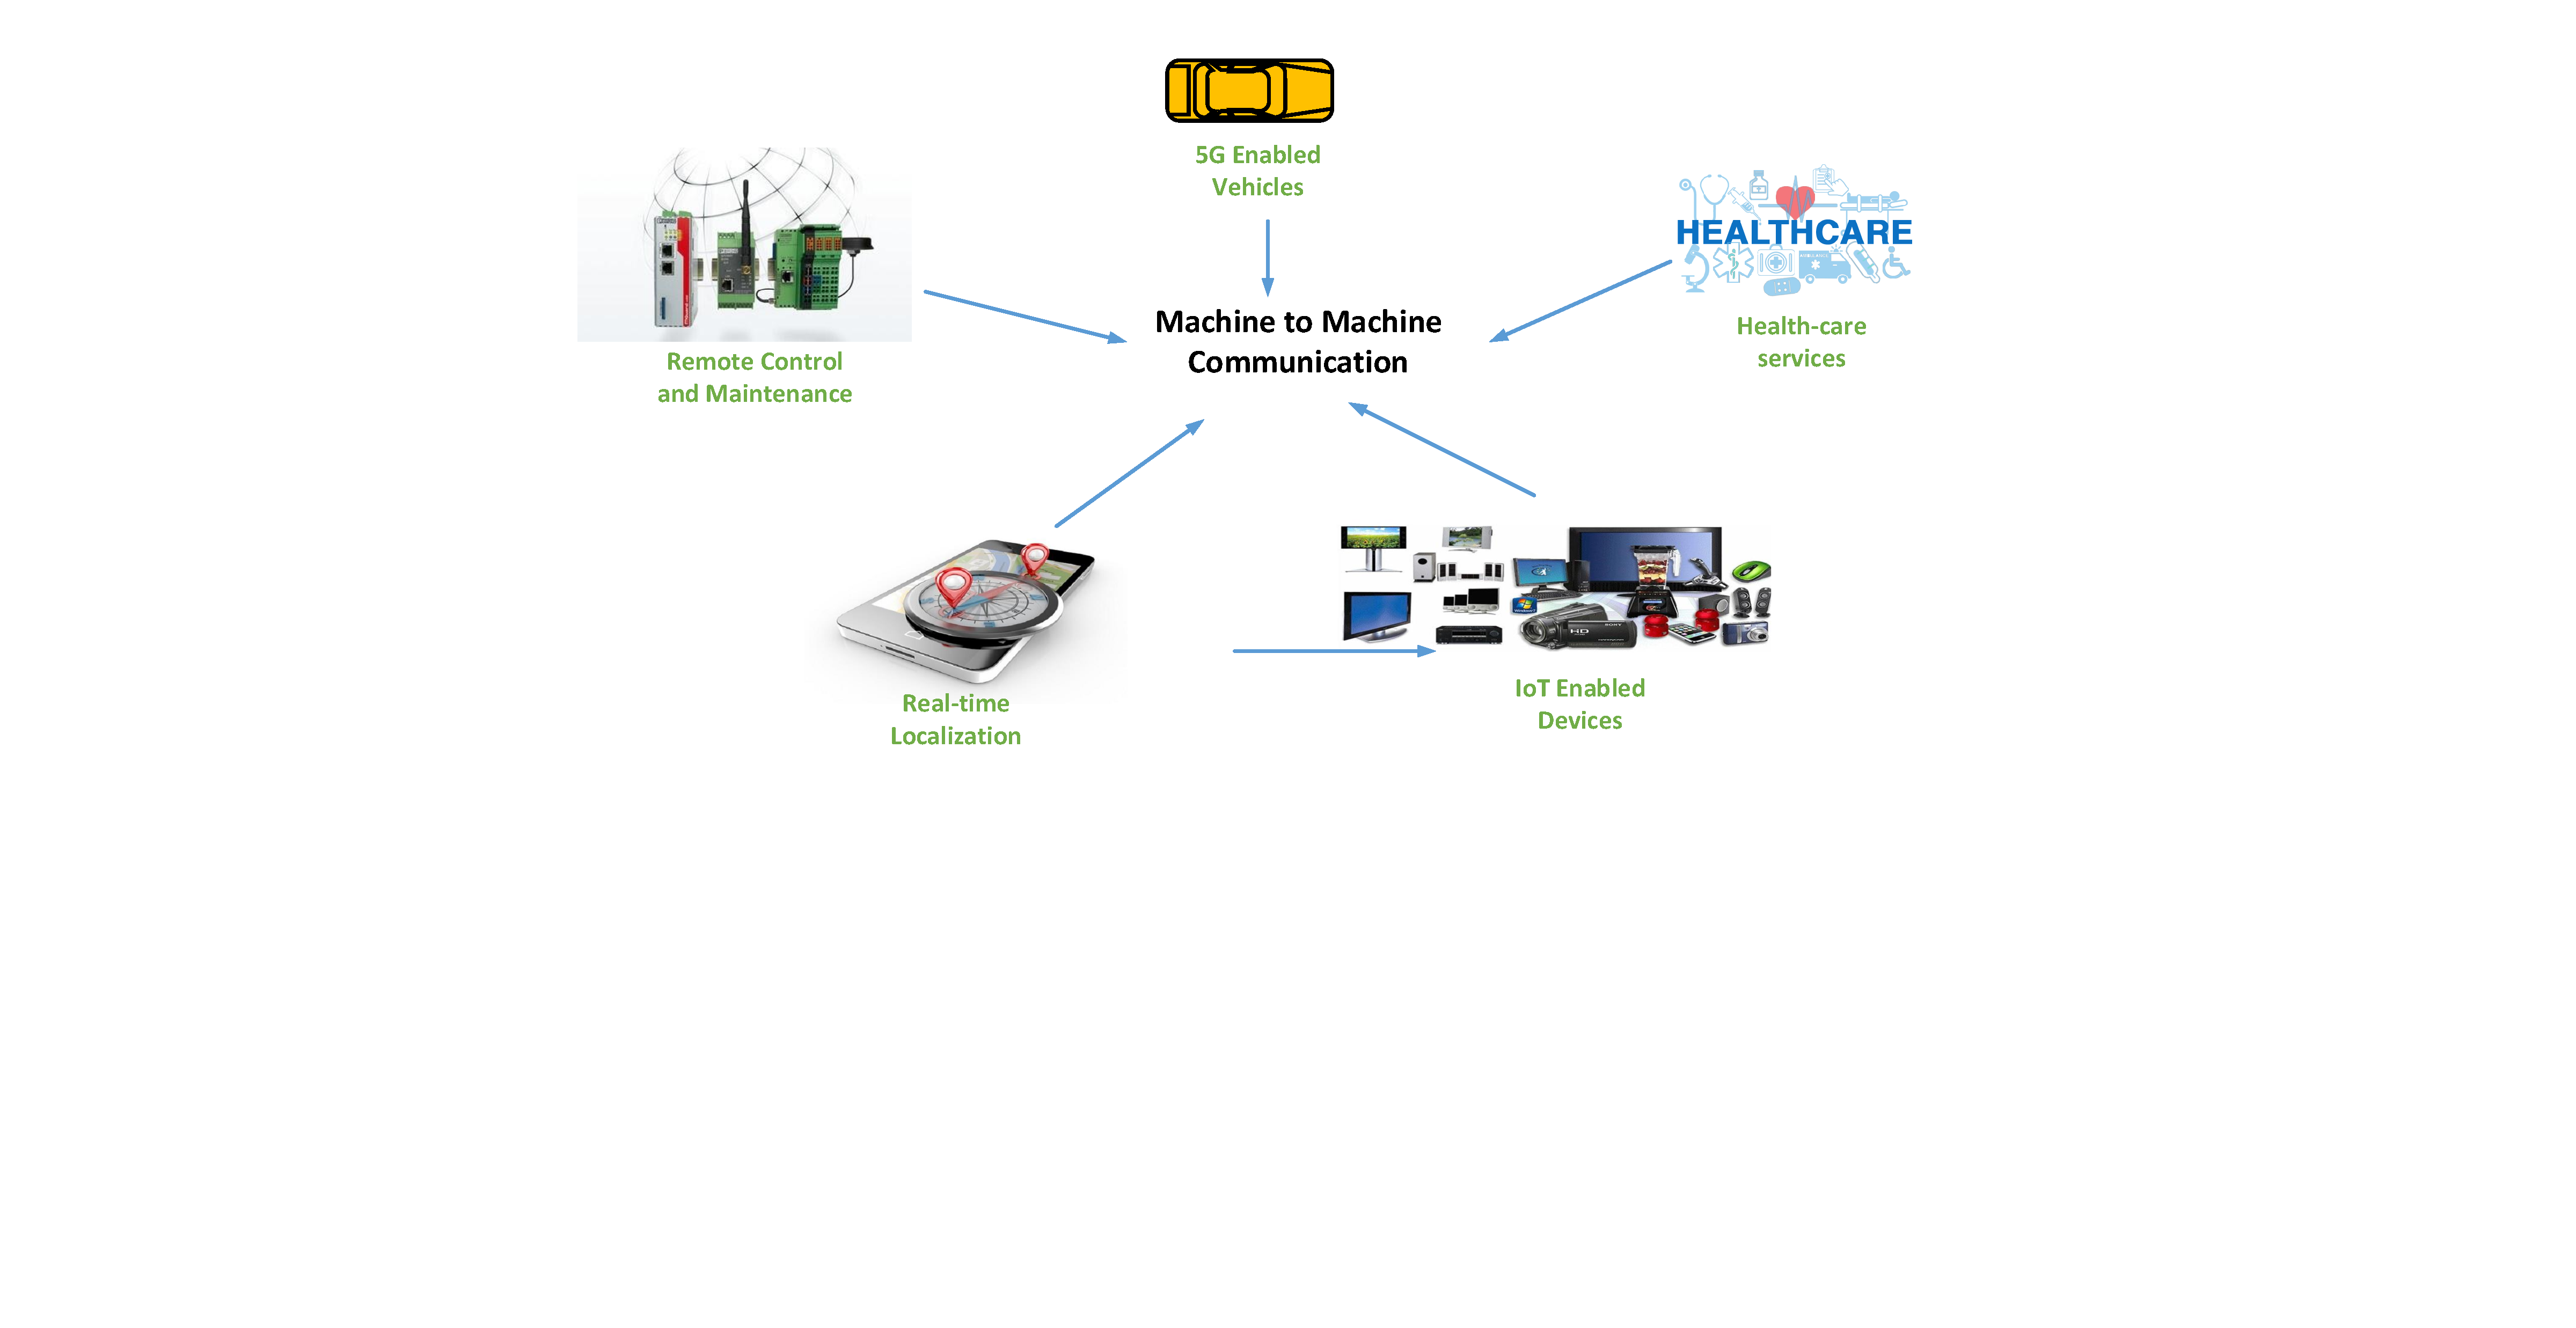
\includegraphics[width=\textwidth,keepaspectratio]{images/Gill/5G/device2device.eps}
	\caption{Machine-to-Machine communication paradigm in 5G Cellular System.}
	\label{d2d}
\end{figure}

Implementing these requirements for 5G system, new communication paradigms needs to be developed at network and physical layer. Figure~\ref{d2d} shows the machine-to-machine communication and how it helps in integrating devices which can be used in health care, localization, vehicular communication, remote maintenance and consumer electronics. In the future standardization of the  5G  networks, the M2M communication is  recognized as one of the key technologies that will support the 5G architecture. As a consequence of this proliferation of M2M technology, large numbers of devices will produce huge amount of irregular data and significantly higher capacity of cellular networks will be needed, in terms of spectrum, power control as well as the number of devices serviced simultaneously. For next generation 5G system, it would be common to have situations where devices will be in close proximity to each other and would like to wirelessly share data like videos, images, etc. or would like to interact for gaming, social networking. If these communication scenarios are handled by simply connecting through the network it can lead to various inefficiencies at various levels. The reason is that cellular networks were primarily designed to support mobile devices with a large amount of data to transmit, whereas most M2M  communications are duty-cycling and  delay-tolerant with small data packets between stationary terminals~\cite{laya2014random}. Thus,  connecting a massive  number  of  M2M  devices  directly  with  cellular networks will saturate uplink traffic easily~\cite{chen2014survey}. In this context, non-cellular connections should serve as important supplement and extension to cellular networks. Some of the challenges of connecting the devices via cellular networks are:

\begin{itemize}
\item Multi-hopping is used to reach destination which otherwise requires fundamentally a single hop. This entails a multi-fold waste of signaling resources as well as higher latency.

\item Huge amount of transmit power is consumed in uplink( fraction of a watt) and downlink( several watts) for data communication which can be easily achieved by milli-watts of power. This leads to unnecessary levels of battery drainage and interference to all other devices occupying the same signaling resources in near proximity.

\item Propagation path-losses to the base stations are much stronger than direct link to the device, hence the corresponding spectral inefficiencies are also lower.
\end{itemize}

It is pretty evident that M2M has huge potential to handle single hop inter device communication more efficiently but these task could be offloaded to other radio access technologies such as Bluetooth, ultra-wide band (UWB) or Zigbee. The applications requiring a mixture of low-latency and high data rates for e.g. interaction between users via augmented reality could be more apt for 5G M2M communication system. In particular, machine-to-machine is as an important enabler for applications requiring low latency, especially in future network deployments utilizing baseband centralization and radio virtualization. There are still various research challenges which need to be taken care of before we can integrate this technology in 5G cellular communication system. The devices for M2M communication need to be designed from both hardware and protocol perspective by providing the needed flexibility at both the PHY and MAC layers. Research needs to be conducted for possible extra overheads for control and channel estimation and also accessing of true net gains associated with M2M mode. And finally, accurate simulation and experimental test-beds needs to be designed for testing M2M communication.

\section{Leaky Coaxial Cable for LTE-R}
Leaky Coaxial Cable (LCX)~\cite{n1974leaky} is an antenna technology designed to deliver radio services in tunnel environment. It consists of small periodic slots to allow radio frequency (RF) signals to escape which act as extended antenna elements. LCX cables were invented to provide the uniform signal coverage in underground mine where radio coverage was very limited due to the geography of the mines. Recently, leaky coaxial cables have been widely used in the field of railway communication especially in tunnels. Leaky feeders are
constructed from coaxial cable where the outer shield has a series of holes with different shapes and different distances among them. The coaxial cable is usually about hundreds of metres long and can be fixed through a building or a tunnel offering radio radiation in a way that would require many individual omni-directional antennae. So far,they have been only used to supplement the direct wireless communication system between a BS and trains, mostly transmitting voice signals. Nowadays, they are being used as an alternative solution to distributed antenna systems in indoor environments like commercial buildings~\cite{motley1983directed,saleh1987distributed} and university buildings, high speed trains, cars, etc. The LCX radio system is almost noise free and has enough bandwidth to support multiple RF signals carrying voice and data simultaneously. Figure~\ref{fig:leakcoax} shows the conventional leaky coaxial cable along x-axis with periodic radiating slots and wave propagation along z-axis. Generally, it consists of three parts: inner conductor, dielectric material and inner conductor. LCX has a dual functionality i.e. they can transmit and receive RF signals using their slots. The frequency range for a leaky cable is given by~\cite{cao1999radio}:
\begin{equation}
\dfrac{c}{\sqrt{\varepsilon_r-1)}d}\geq f \leq \dfrac{c}{\sqrt{\varepsilon_r}+1)d}
\end{equation}

\begin{figure}[!ht]
\label{fig:leakcoax}
\centering
\includegraphics[width=\textwidth,keepaspectratio]{images/Gill/lte_figs/leakycoax.eps} 
\caption{Leaky Coaxial Cable}
\end{figure}

A radio system based on LCX has been deployed in Japan for high speed railways ''Series N700''~\cite{takatsu2007history} to connect the train to ground network. Wi-Fi access points are chosen for in-train communications with peak data rates of 2 Mbps for uplink and downlink. Although current technologies can provide wireless communication services in HSTs, the capacity of communication system is very low (1--4 Mbps). These data rates are insufficient for next generation wireless communication system where the peak data rates of 0.5 -- 5 Gbps are expected. LTE-R communication system can be implemented for achieving high data rates but it cannot be achieved by using conventional cellular system. The penetration loss due to tunnel walls is very high and secondly, the fast moving trains causes large Doppler shifts leading to poor connectivity due to retransmissions. Hence, leaky coaxial cable is the best candidate for achieving extensive internet access inside a tunnel environment for high speed railways.

\section{summary}
A radio system based on LCX has been deployed in Japan for high speed railways ''Series N700''~\cite{takatsu2007history} to connect the train to ground network. Wi-Fi access points are chosen for in-train communications with peak data rates of 2 Mbps for uplink and downlink. Although current technologies can provide wireless communication services in HSTs, the capacity of communication system is very low (1--4 Mbps). These data rates are insufficient for next generation wireless communication system where the peak data rates of 0.5 -- 5 Gbps are expected. LTE-R communication system can be implemented for achieving high data rates but it cannot be achieved by using conventional cellular system. The penetration loss due to tunnel walls is very high and secondly, the fast moving trains causes large Doppler shifts leading to poor connectivity due to retransmissions. Hence, leaky coaxial cable is the best candidate for achieving extensive internet access inside a tunnel environment for high speed railways.